\section{INTRODUÇÃO}

Este relatório apresenta o trabalho final da disciplina de Estrutura de Dados II (EDA2), feito por Vinicius Moreira Krüger, Gustavo Bada Zanatta, Lucas da Silva e Gustavo Holderegger, estudantes de Ciência da Computação da UDESC, em Joinville, no semestre de 2026/2.

O objetivo do trabalho é medir o esforço das operações de adição e de remoção de chaves em cinco árvores balanceadas: AVL, rubro-negra e árvore B com ordem 1, 5 e 10. O esforço medido conta também o balanceamento que cada árvore faz depois da operação. Os testes usam conjuntos de 1 a 10.000 chaves aleatórias, que representam o caso médio, e para cada tamanho foi feita a média de 10 conjuntos diferentes.

\section{ESTRUTURAS AVALIADAS}

A árvore AVL é uma árvore binária de busca em que, em todo nó, a altura da subárvore da esquerda e a da direita podem diferir em no máximo 1. Essa diferença é o fator de balanceamento. Depois de uma adição ou remoção, a árvore sobe atualizando as alturas e, quando algum nó fica com fator 2 ou $-2$, faz uma rotação simples ou dupla.

A árvore rubro-negra também é uma árvore binária de busca, mas cada nó é vermelho ou preto. A raiz é preta, um nó vermelho não pode ter filho vermelho e todos os caminhos até as folhas têm a mesma quantidade de nós pretos. Quando uma operação quebra alguma dessas regras, a árvore troca cores e, se precisar, faz rotações.

A árvore B guarda várias chaves em cada nó. Com ordem $d$, cada nó tem entre $d$ e $2d$ chaves (a raiz pode ter menos) e todas as folhas ficam no mesmo nível. Na adição, quando um nó passa de $2d$ chaves, ele é dividido e a chave do meio sobe para o pai. Na remoção, quando um nó fica com menos de $d$ chaves, ele pega uma chave emprestada de um irmão ou é juntado com ele. Com ordem 1 os nós têm de 1 a 2 chaves, com ordem 5 têm de 5 a 10 e com ordem 10 têm de 10 a 20.

Nas três árvores a altura cresce de forma logarítmica com a quantidade de chaves. Por isso, adicionar ou remover uma chave custa $O(\log n)$.

\section{IMPLEMENTAÇÃO}

\subsection{ORGANIZAÇÃO DO CÓDIGO}

O trabalho foi feito em C e está dividido em três pastas: \texttt{codigo}, \texttt{resultados} e \texttt{relatorio}. Na pasta \texttt{codigo}, cada árvore tem um arquivo \texttt{.c} e um \texttt{.h}: \texttt{avl}, \texttt{rubronegra} e \texttt{arvoreb}. O \texttt{main.c} junta as três árvores e roda o experimento inteiro. O script \texttt{graficos.py}, em Python, lê os resultados e gera os gráficos.

Os códigos passados em aula foram usados como base. Eles só tinham a adição, então escrevemos a remoção das três árvores seguindo o mesmo jeito de programar. Também corrigimos alguns pontos:

\begin{itemize}
\item na AVL, a escolha da rotação usava \texttt{fb(filho) > 0}. Na remoção o filho pode ficar com fator 0, e nesse caso a rotação certa é a simples, então a condição passou a ser \texttt{>= 0} (e \texttt{<= 0} do outro lado);
\item na rubro-negra, a raiz começava como \texttt{NULL}, mas o resto do código usa o nó \texttt{nulo}. Depois de remover todas as chaves a raiz volta a ser o \texttt{nulo}, então ela passou a começar assim também;
\item na árvore B, o vetor de filhos era alocado com \texttt{sizeof(No)}, sendo que ele guarda ponteiros (\texttt{sizeof(No*)}), e a busca dentro da folha era feita duas vezes em cada adição.
\end{itemize}

\subsection{MEDIDA DO ESFORÇO}

O esforço foi medido contando operações, e não tempo, para que o resultado não dependa do computador. Existe uma variável global \texttt{contador} que soma 1 a cada:

\begin{itemize}
\item comparação com uma chave durante a busca;
\item passo na busca do sucessor, na remoção;
\item passo do balanceamento (nó atualizado na subida da AVL ou volta do laço de correção da rubro-negra);
\item rotação (a dupla conta duas);
\item divisão, empréstimo ou junção de nós na árvore B e cada chave que precisa ser movida dentro de um nó.
\end{itemize}

\subsection{EXPERIMENTO}

Na primeira execução, o programa gera 10 conjuntos de 10.000 chaves aleatórias e diferentes com a função \texttt{rand} e salva tudo no arquivo \texttt{chaves.csv}, com um conjunto por coluna. Nas execuções seguintes ele só lê esse arquivo, então as chaves não mudam e as cinco árvores sempre recebem exatamente os mesmos dados.

Para cada tamanho $N$ (primeiro $N = 1$ e depois de 10 em 10 até 10.000) e para cada um dos 10 conjuntos, o programa cria as cinco árvores, adiciona as $N$ primeiras chaves do conjunto e depois remove essas mesmas chaves, na mesma ordem em que foram adicionadas, até a árvore ficar vazia. Como as chaves são aleatórias, a ordem de remoção também é aleatória.

O valor salvo para cada $N$ é o esforço médio por operação: o total contado dividido pelas $N$ operações e pelos 10 conjuntos. Escolhemos mostrar a média por operação, e não o esforço total para adicionar ou remover as $N$ chaves, porque assim o custo de cada operação, que é o que a complexidade $O(\log n)$ descreve, aparece direto no gráfico. O esforço total é esse valor multiplicado por $N$ e cresce na ordem de $N \log N$. Os resultados ficam nos arquivos \texttt{resultado\_adicao.csv} e \texttt{resultado\_remocao.csv}, na pasta \texttt{resultados}, com uma coluna para cada árvore. Ao final, o programa também mostra a altura de cada árvore com as 10.000 chaves do primeiro conjunto.

\section{COMPILAÇÃO E EXECUÇÃO}

Os programas foram compilados pela linha de comando, sem uso de IDE. Os comandos devem ser executados dentro da pasta \texttt{codigo}:

\begin{flushleft}
\ttfamily\small
\noindent gcc -Wall -Wextra -std=c11 -O2 main.c avl.c rubronegra.c arvoreb.c -o main\\
./main
\end{flushleft}

A execução completa levou 3 minutos no nosso computador. Depois que ela termina, os gráficos são gerados com Python 3:

\begin{flushleft}
\ttfamily\small
\noindent python3 -m pip install pandas matplotlib\\
python3 graficos.py
\end{flushleft}

O código foi compilado no Ubuntu 24.04 usando GCC, sem avisos com as opções descritas acima. Antes de medir, conferimos que as cinco árvores continuavam corretas depois de cada adição e de cada remoção, e também rodamos o código com o AddressSanitizer, sem nenhum erro de memória.

\section{RESULTADOS}

As Figuras~\ref{fig:adicao} e~\ref{fig:remocao} mostram o esforço médio por operação para cada tamanho de conjunto.

\begin{figure}[htb]
  \centering
  \caption{Esforço médio da adição de chaves}
  \label{fig:adicao}
  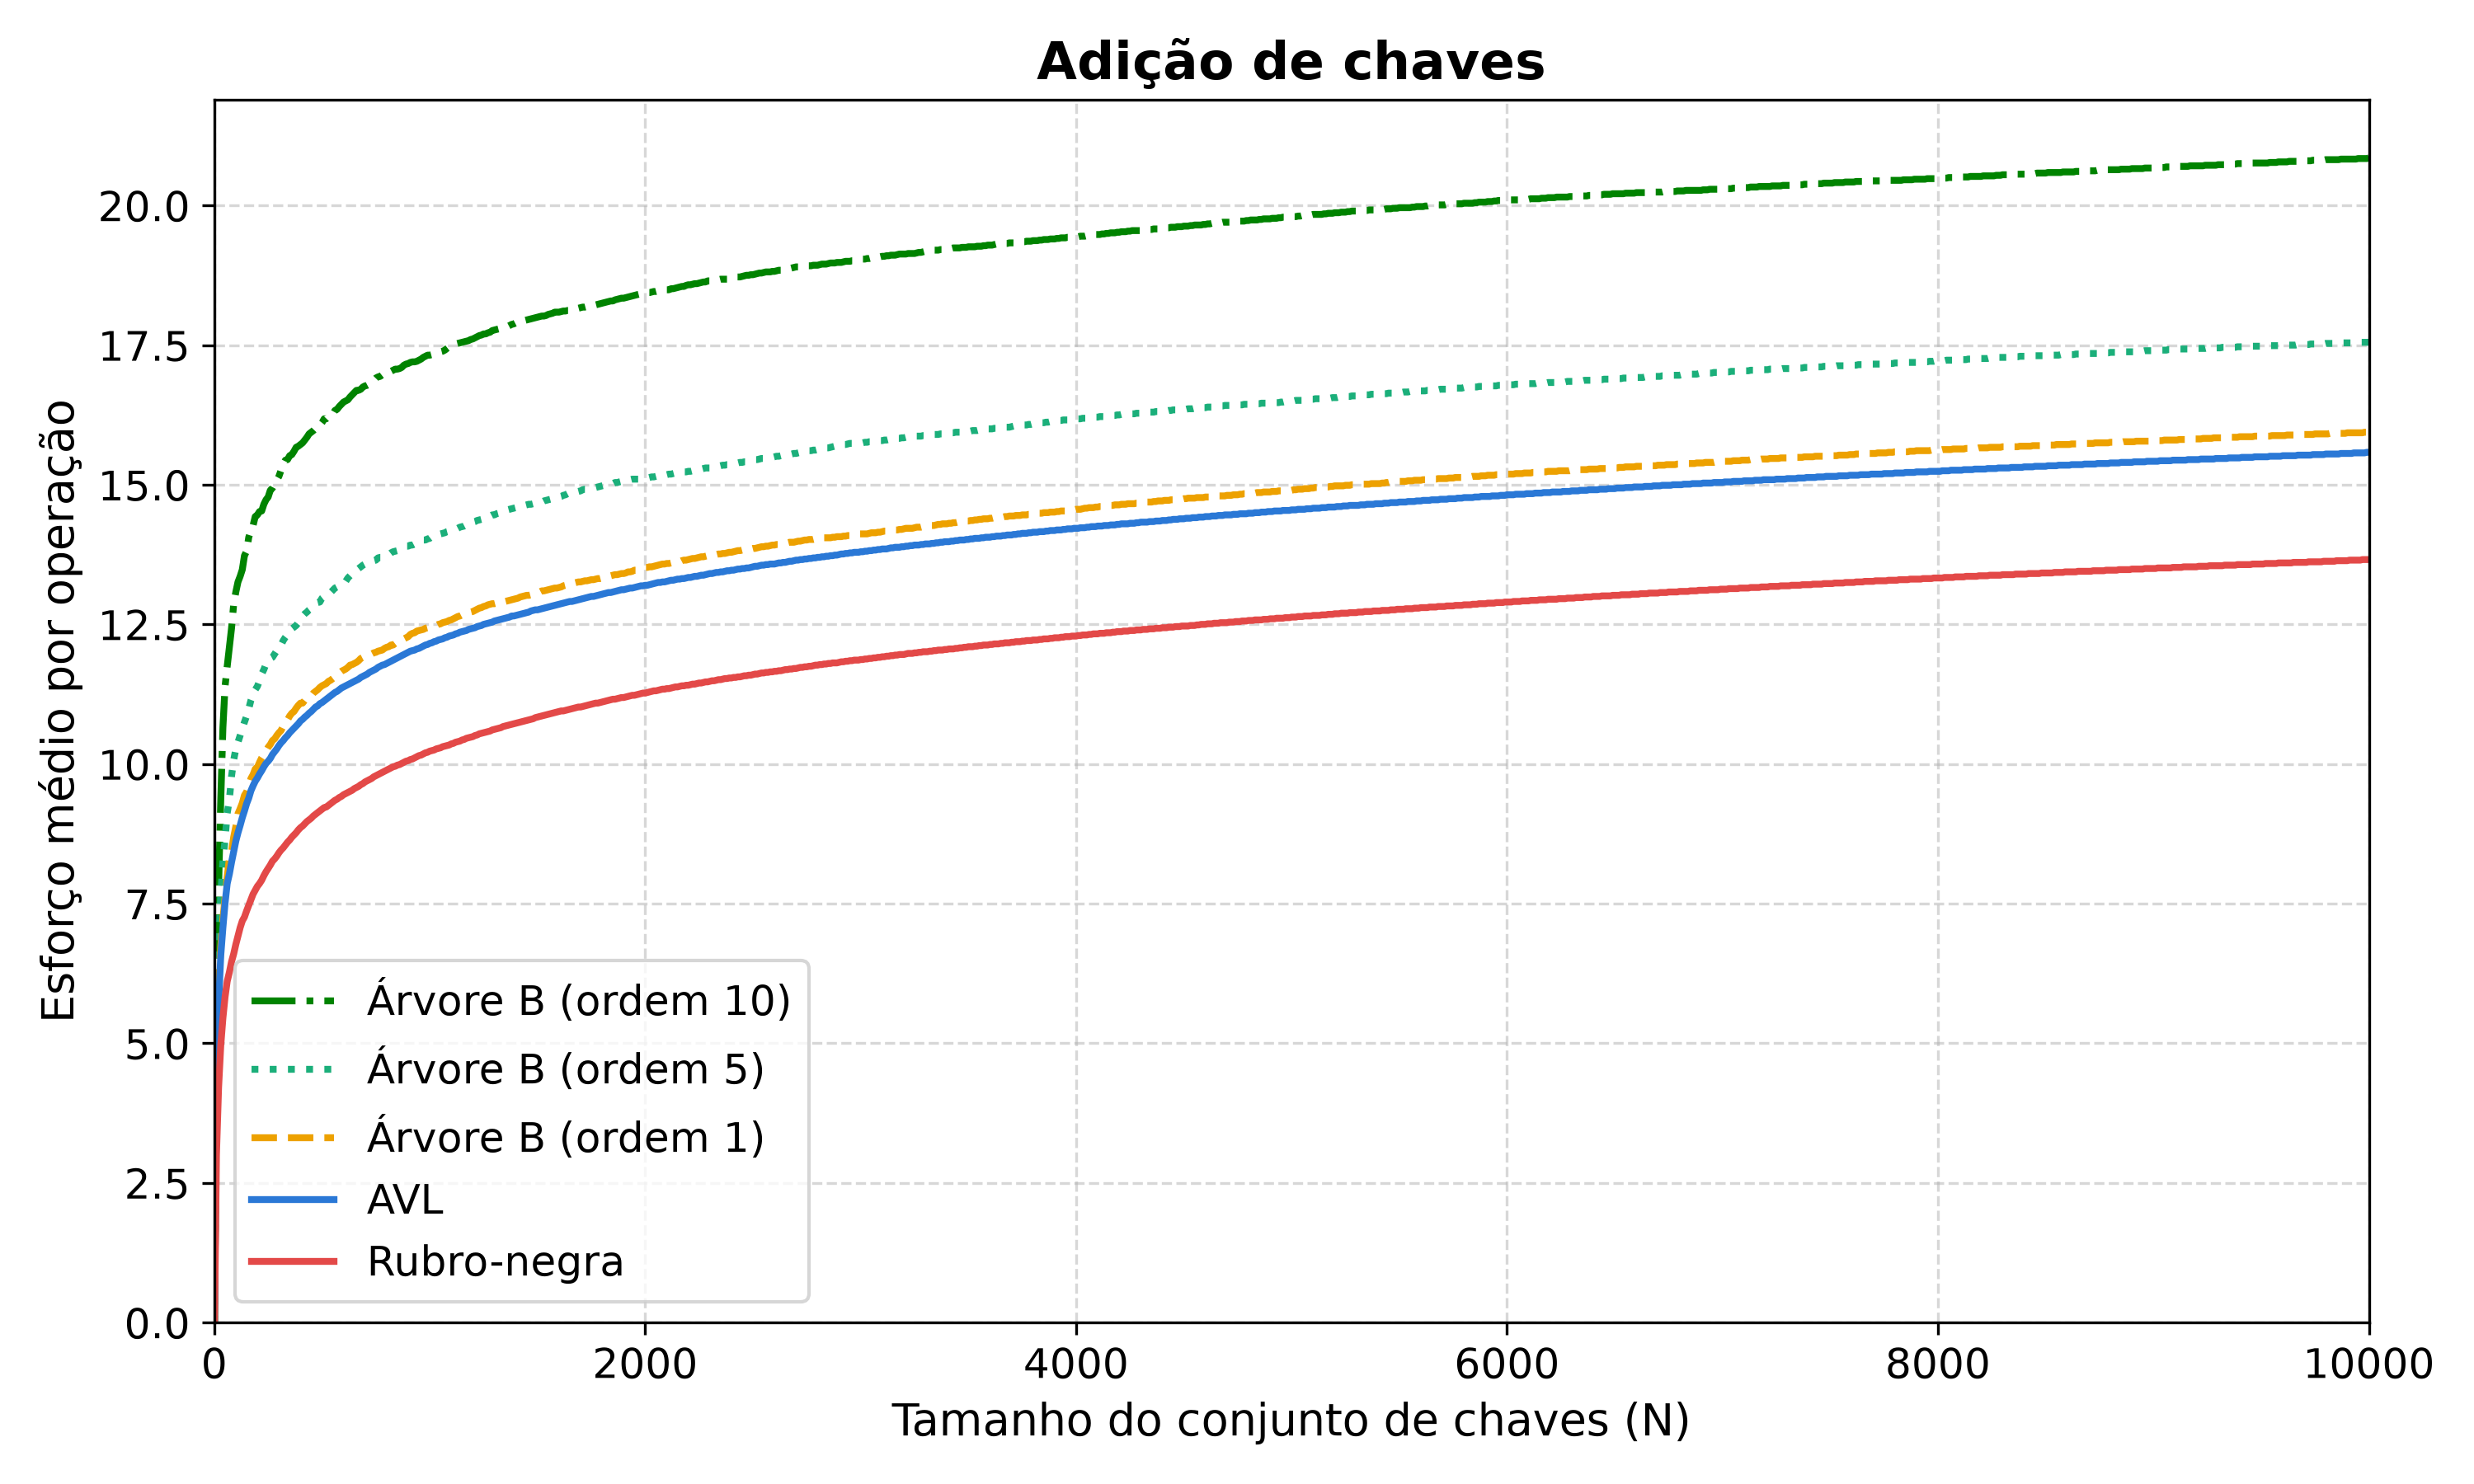
\includegraphics[width=\textwidth]{figuras/grafico_adicao.png}
  \par\vspace{0.15\baselineskip}
  {\footnotesize Fonte: Elaborada pelos autores (2026).\par}
\end{figure}

\begin{figure}[htb]
  \centering
  \caption{Esforço médio da remoção de chaves}
  \label{fig:remocao}
  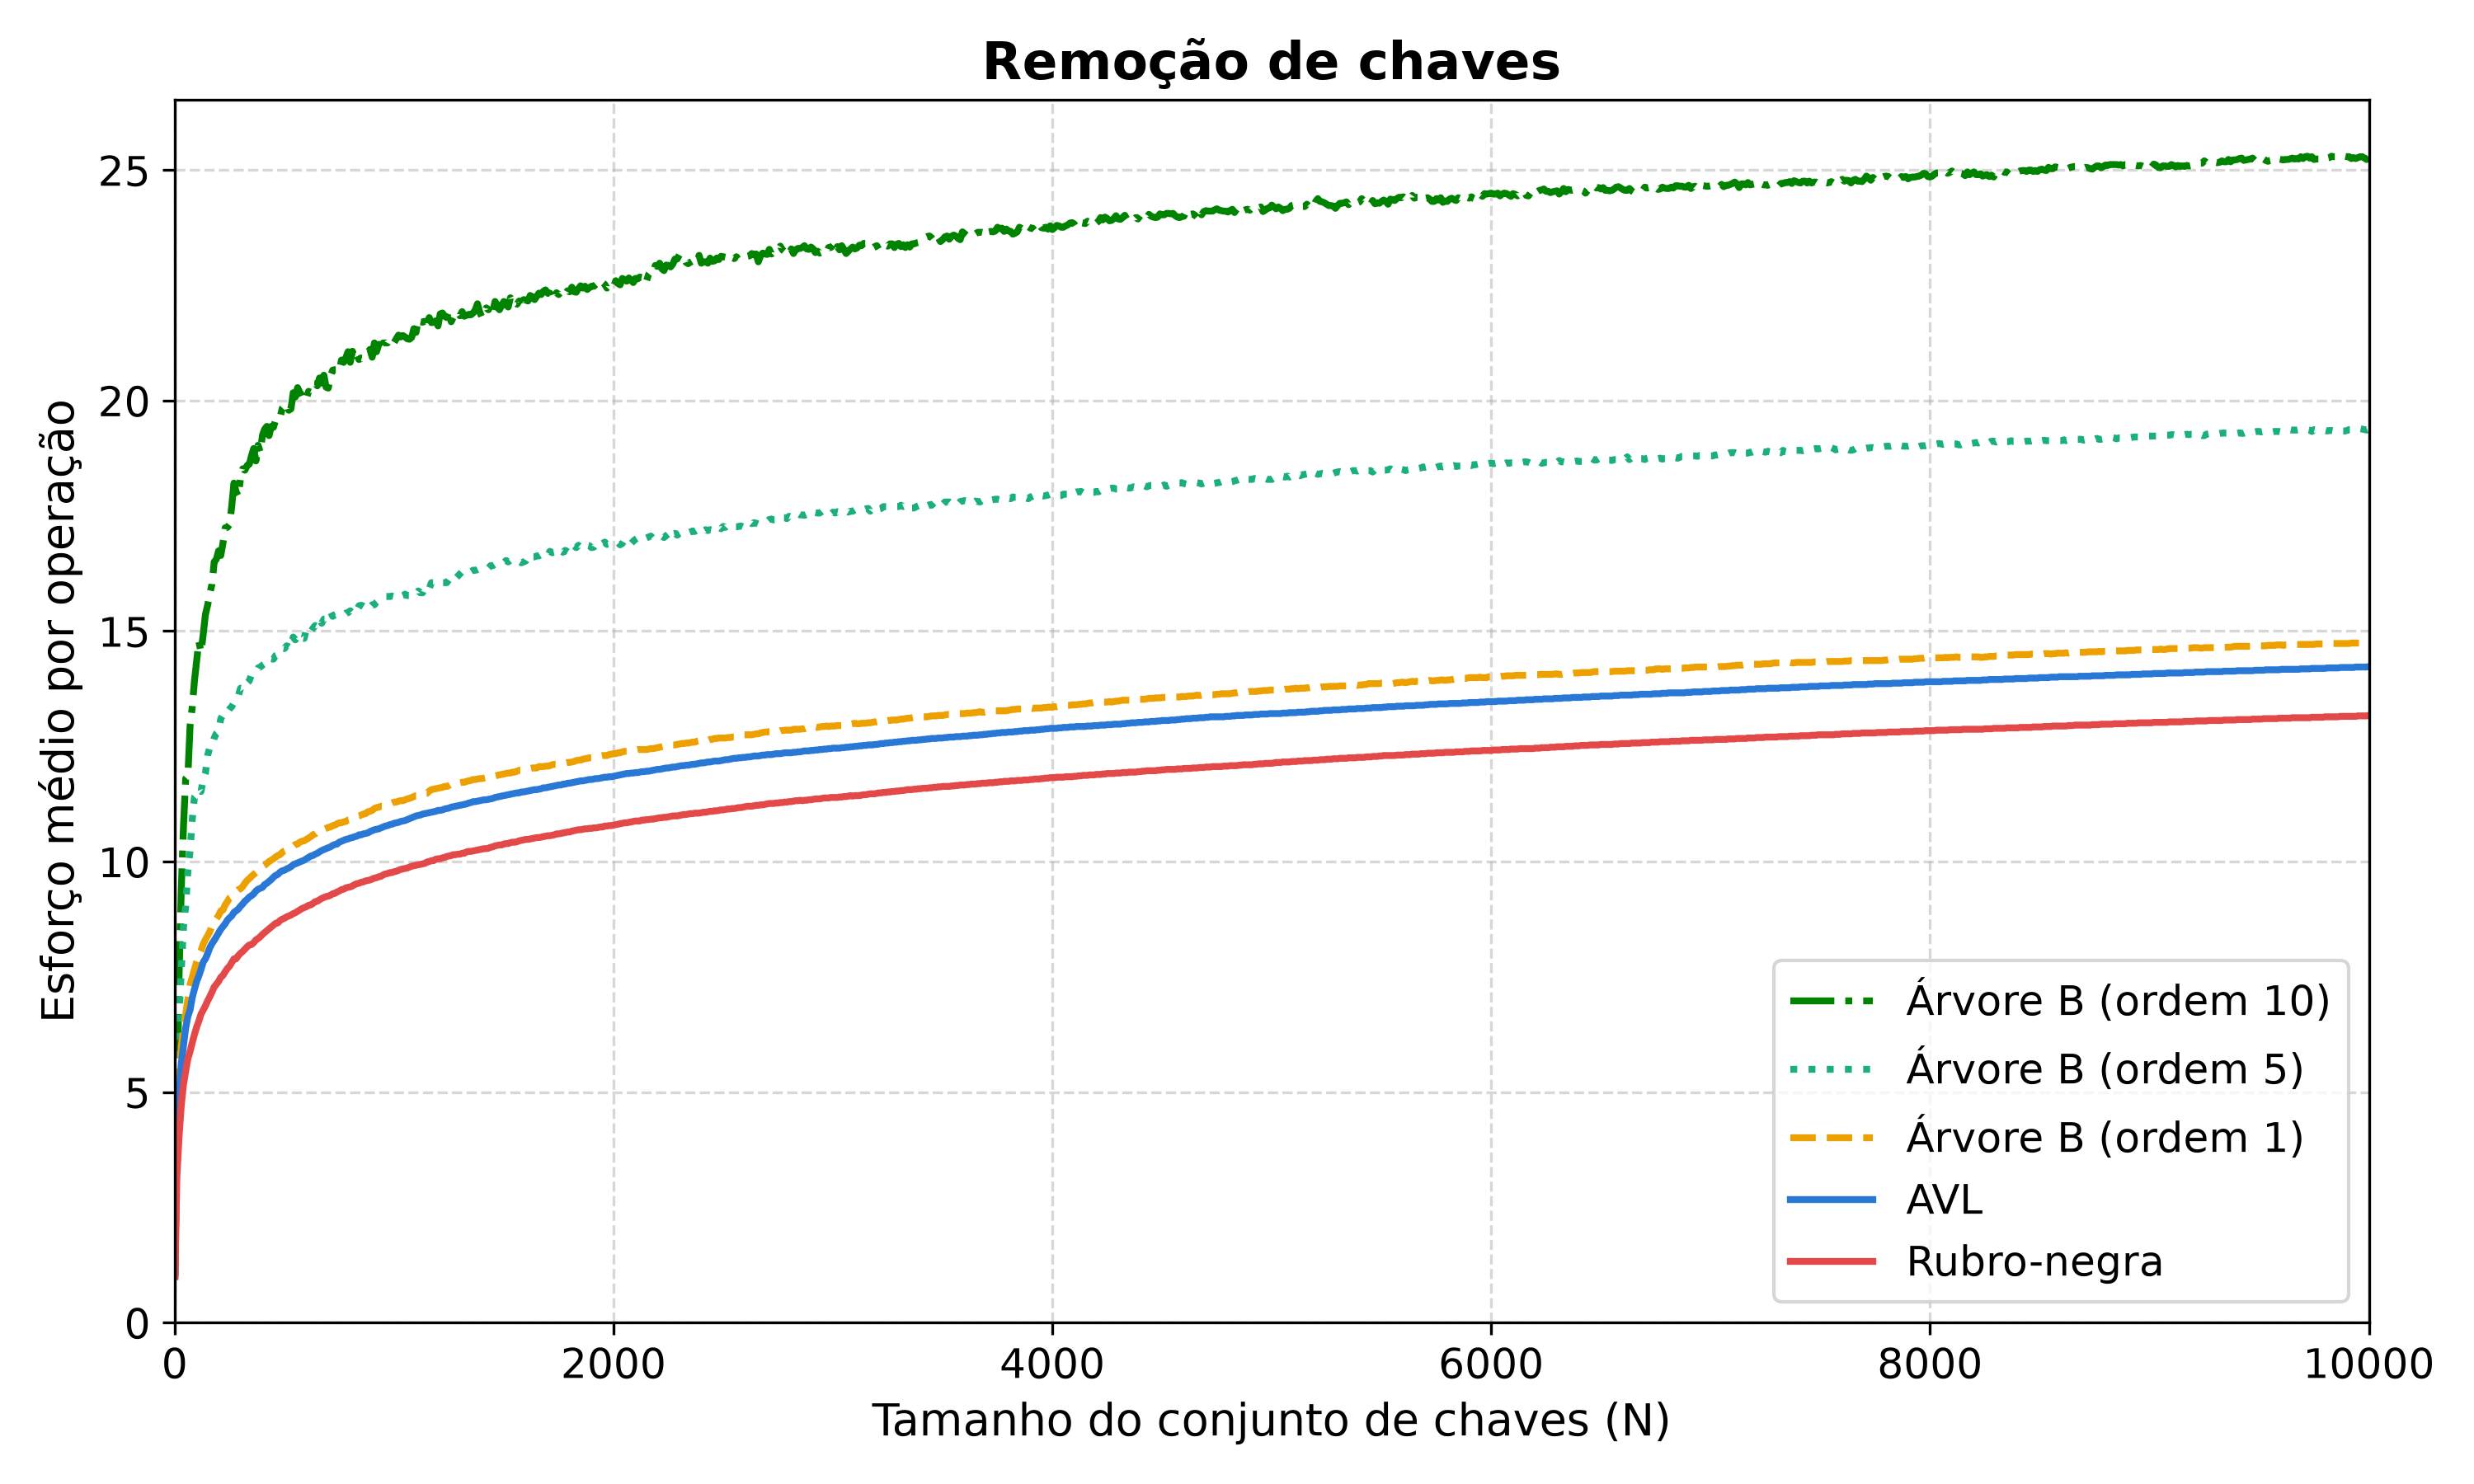
\includegraphics[width=\textwidth]{figuras/grafico_remocao.png}
  \par\vspace{0.15\baselineskip}
  {\footnotesize Fonte: Elaborada pelos autores (2026).\par}
\end{figure}

A Tabela~\ref{tab:resultados} mostra os valores para 1.000 e 10.000 chaves e a altura de cada árvore com as 10.000 chaves do primeiro conjunto.

\begin{table}[htb]
  \centering
  \caption{Esforço médio por operação e altura das árvores}
  \label{tab:resultados}
  \begin{tabular}{@{}lccccc@{}}
    \toprule
    & \multicolumn{2}{c}{\textbf{Adição}} & \multicolumn{2}{c}{\textbf{Remoção}} & \\
    \cmidrule(lr){2-3}\cmidrule(lr){4-5}
    \textbf{Árvore} & \textbf{1.000} & \textbf{10.000} & \textbf{1.000} & \textbf{10.000} & \textbf{Altura} \\
    \midrule
    AVL                & 12,16 & 15,58 & 10,83 & 14,23 & 16 \\
    Rubro-negra        & 10,23 & 13,66 & 9,78 & 13,17 & 16 \\
    B, ordem 1         & 12,45 & 15,94 & 11,29 & 14,75 & 11 \\
    B, ordem 5         & 14,04 & 17,55 & 15,75 & 19,38 & 5 \\
    B, ordem 10        & 17,32 & 20,85 & 21,26 & 25,27 & 4 \\
    \bottomrule
  \end{tabular}
  \par\vspace{0.2\baselineskip}
  {\footnotesize Fonte: Elaborada pelos autores (2026).\par}
\end{table}

\section{DISCUSSÃO DOS RESULTADOS}

As cinco curvas têm o formato esperado para $O(\log n)$: sobem rápido no começo e depois vão ficando quase planas. Na adição da AVL, por exemplo, o esforço médio foi de 4,16 com 10 chaves, 8,62 com 100, 12,16 com 1.000 e 15,58 com 10.000. A cada dez vezes mais chaves, cada operação ficou só umas 3 ou 4 operações mais cara, que é bem perto de $\log_2 10 \approx 3{,}3$. Se o crescimento fosse linear, o esforço teria sido multiplicado por dez a cada passo. No começo dos gráficos as linhas oscilam um pouco, porque com poucas chaves a média depende muito de quais chaves foram sorteadas.

A rubro-negra teve o menor esforço nas duas operações. Ela e a AVL ficaram com a mesma altura, então a busca custa quase o mesmo nas duas, e a diferença está no balanceamento. A AVL recalcula a altura de cada nó no caminho de volta, enquanto a rubro-negra só entra no laço de correção quando o pai do nó inserido ou removido é vermelho, e na maioria das vezes resolve trocando poucas cores. O número de rotações foi parecido nas duas: com 10.000 chaves, cerca de 0,7 por adição na AVL e 0,6 na rubro-negra, e cerca de 0,4 por remoção nas duas.

A árvore B de ordem 1 ficou perto da AVL. Nas ordens 5 e 10 a árvore fica bem mais baixa, com 5 e 4 níveis, mas o esforço aumentou. Isso acontece porque, mesmo com menos níveis, a busca binária dentro de cada nó faz a quantidade de comparações continuar parecida. Além disso, para manter as chaves em ordem dentro do nó, cada adição ou remoção precisa deslocar várias chaves, e isso pesa mais quanto maior é o nó.

Na AVL, na rubro-negra e na árvore B de ordem 1, remover foi um pouco mais barato que adicionar, porque a chave removida é encontrada no próprio nó em que está e nem sempre é preciso descer até o fim da árvore. Nas ordens 5 e 10 aconteceu o contrário: além dos deslocamentos, os nós que ficam com poucas chaves precisam de empréstimos e junções com frequência, e cada um deles move várias chaves.

Isso não quer dizer que a árvore B seja ruim. Ela foi pensada para dados guardados em disco, onde ler um nó demora muito mais do que comparar chaves na memória. Nesse caso o que importa é a quantidade de nós visitados, e ter 4 níveis em vez de 16 faz muita diferença. Como neste trabalho tudo fica na memória, essa vantagem não aparece.

\section{CONSIDERAÇÕES FINAIS}

As cinco árvores mostraram o comportamento esperado de $O(\log n)$ por operação, já contando o balanceamento. Na memória, a rubro-negra teve o menor esforço, seguida pela AVL e pela árvore B de ordem 1, que ficaram próximas. As árvores B de ordem 5 e 10 foram as que mais gastaram, apesar de serem as mais baixas, porque o trabalho passa a ficar dentro dos nós.

No geral, a rubro-negra é uma boa escolha quando há muitas adições e remoções, a AVL, que tem um balanceamento mais rígido, é interessante quando há mais buscas do que alterações, e a árvore B vale mais a pena quando os dados ficam em disco.
